\chapter{Realisierung}

In diesem Kapitel werden die zentralen Komponenten der Systemarchitektur vorgestellt. Es beginnt mit dem modular aufgebauten Backend auf Basis von Spring Boot, gefolgt von der Struktur und Internationalisierung des Frontends mit React. Abschließend wird das Datenbankmodell erläutert, einschließlich der Persistenzlogik mit Spring Data und Hibernate.

\section{Backend-Architektur}\index{Backend-Architektur}
 
Das Backend basiert auf Spring Boot und folgt einer klar strukturierten, modularen Architektur. Beschrieben werden der Einstiegspunkt, die Paketstruktur sowie die eingesetzte Teststrategie zur Sicherstellung der Codequalität.

\subsection{Projektinitialisierung und Startklasse}\index{Projektinitialisierung}

Spring Boot vereinfacht die Entwicklung von Java-basierten Webanwendungen durch konventionsbasierte und automatisierte Projektkonfiguration. Dieses Framework bietet eine standardisierte Struktur, automatisches Abhängigkeitsmanagement und integrierte Komponenten, die den Entwicklungsprozess erheblich beschleunigen.

\noindent In diesem Abschnitt wird die Struktur des Projekts erläutert, wobei der Schwerpunkt auf der Projektinitialisierung, den zentralen Einstiegspunkt der Anwendung sowie wesentliche Konfigurationsmechanismen liegt.
\begin{itemize}
	\item \textbf{Projektinitialisierung (Spring Initializr):} Die Anwendung \textit{LibraNova} wurde mithilfe des Online-Tools \textit{Spring Initializr} (\url{https://start.spring.io/}) erzeugt. Dieses Tool ermöglicht die einfache Auswahl von Projektparametern wie Abhängigkeiten, Java-Version und Build-Tool (z.\,B. Maven oder Gradle) und generiert eine startbereite Projektstruktur inklusive grundlegender Dateien und Verzeichnisse.
	
	\item \textbf{Einstiegspunkt der Anwendung – Main-Klasse:} Die zentrale Einstiegsklasse der Anwendung befindet sich im \texttt{src/main/java}-Verzeichnis und enthält die \texttt{main}-Methode. Sie ist mit der Annotation \texttt{@SpringBootApplication} versehen, welche drei wichtige Spring-Annotationen kombiniert:
	\begin{itemize}
		\item \texttt{@Configuration} – Kennzeichnet die Klasse als Quelle für Bean-Definitionen.
		\item \texttt{@EnableAutoConfiguration} – Aktiviert die automatische Konfiguration basierend auf den eingebundenen Abhängigkeiten.
		\item \texttt{@ComponentScan} – Ermöglicht das automatische Auffinden von Komponenten, Services und Repositories im angegebenen Paket und dessen Unterpaketen.
	\end{itemize}
	
	Nachfolgend \ref{lst:springboot-main} ist der Quellcode der Main-Klasse dargestellt:
	
	\begin{lstlisting}[language=Java, caption=Einstiegspunkt der Spring Boot Anwendung, label=lst:springboot-main, breaklines=true]
		@SpringBootApplication
		public class SpringBootLibraryApplication {
			
			public static void main(String[] args) {
				SpringApplication.run(SpringBootLibraryApplication.class, args);
			}
			
		}
	\end{lstlisting}

  \noindent \textit{Erläuterung der Main-Klasse:}
  \begin{itemize}
  	\item \texttt{@SpringBootApplication}: Diese Annotation bündelt die Konfiguration, Auto-Konfiguration und Komponentensuche in einer einzigen Annotation und ist der zentrale Startpunkt für die Spring-Boot-Anwendung.
  	\item \texttt{public class SpringBootLibraryApplication}: Definition der Hauptklasse, die die Anwendung repräsentiert.
  	\item \texttt{public static void main(String[] args)}: Die Main-Methode dient als Einstiegspunkt der Java-Anwendung. Sie wird beim Programmstart aufgerufen.
  	\item \texttt{SpringApplication.run(...) }: Diese Methode startet den eingebetteten Server, initialisiert den Spring Application Context und lädt alle Komponenten, Beans und Konfigurationen.
  \end{itemize}

\item \textbf{Konfiguration über \texttt{application.properties}:} Die Datei \texttt{application.properties} im Verzeichnis \texttt{src/main/resources} enthält zentrale Konfigurationen der Anwendung, wie z.\,B. Datenbankverbindung, REST-Basis-Pfad und andere anwendungsspezifische Einstellungen.

\begin{lstlisting}[language=, caption=Beispielhafte application.properties Datei, label=lst:application-properties, breaklines=true]
	# Name der Anwendung
	spring.application.name=libranova
	
	# Datenbankverbindung (MySQL)
	spring.datasource.url=jdbc:mysql://localhost:3306/libranova_db
	spring.datasource.username=username
	spring.datasource.password=password
	
	# Dialekt von Hibernate
	spring.jpa.properties.hibernate.dialect=org.hibernate.dialect.MySQLDialect
	
	# Basis-REST-Pfad
	spring.data.rest.base-path=/api
\end{lstlisting}

\textit{Erläuterung der wichtigsten Einstellungen:}
\begin{itemize}
	\item \texttt{spring.application.name}: Definiert den Namen der Anwendung, z.\,B. für Logs oder Monitoring.
	\item \texttt{spring.datasource.url}: Verbindungs-URL zur MySQL-Datenbank inklusive Host, Port und Datenbankname.
	\item \texttt{spring.datasource.username}: Benutzername für die Datenbankverbindung.
	\item \texttt{spring.datasource.password}: Passwort für den Datenbankzugang.
	\item \texttt{spring.jpa.properties.hibernate.dialect}: Gibt den SQL-Dialekt für JPA/Hibernate an (hier MySQL).
	\item \texttt{spring.data.rest.base-path}: Legt den Basis-URL-Pfad für automatisch generierte REST-Endpunkte fest (z.\,B. \texttt{/api}).
\end{itemize}

\item \textbf{Eingebetteter Webserver (Tomcat):} Spring Boot integriert standardmäßig einen eingebetteten Webserver (standardmäßig Tomcat). Dadurch kann die Anwendung direkt als eigenständiger Prozess gestartet werden, ohne dass ein separater Webserver installiert oder konfiguriert werden muss \cite{SPRINGBOOT2025b}.
\end{itemize}

\subsection{Modulare Paketstruktur des Backends}\index{Paketstruktur}
Im Folgenden wird die interne Struktur des Backends detailliert betrachtet. Dazu gehört die Aufteilung der Anwendung in verschiedene Pakete, die jeweils eigene Verantwortlichkeiten übernehmen und so zur Übersichtlichkeit und Wartbarkeit beitragen.  

\noindent Eine schematische Übersicht der Paketstruktur ist in \textbf{Abbildung~\ref{fig:package-structure}} unten dargestellt.
\begin{figure}[H]
	\centering
	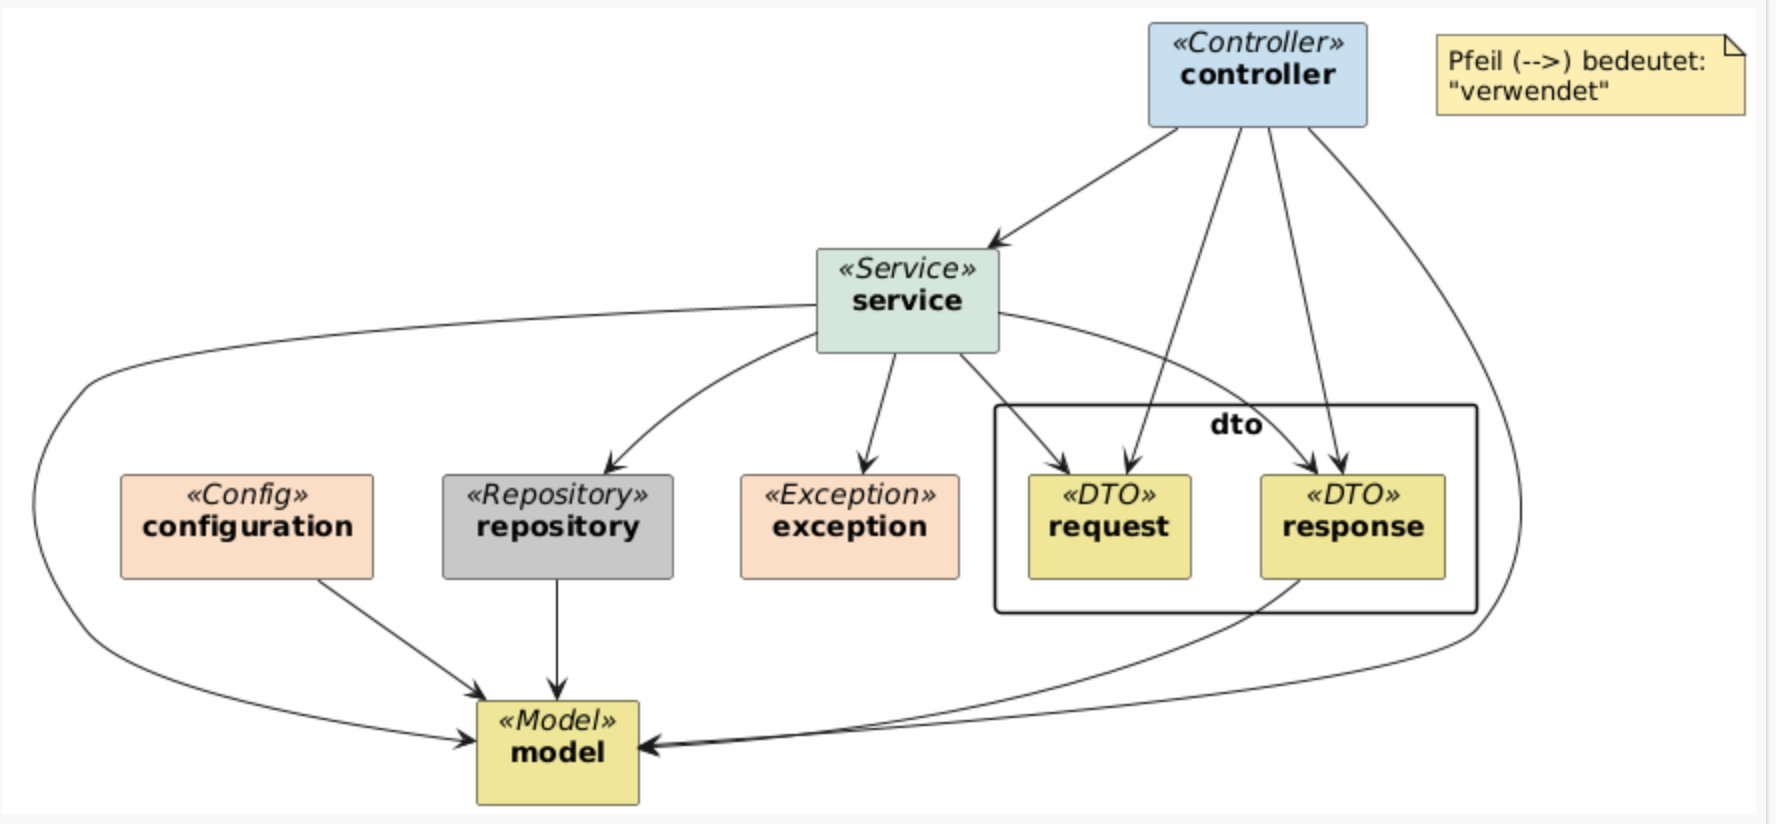
\includegraphics[width=0.99\textwidth]{images/backend_structure.png}
	\caption{Modularer Aufbau des Backends}
	\label{fig:package-structure}
\end{figure} 
\noindent Im Folgenden werden die Pakete und ihre jeweiligen Verantwortlichkeiten beschrieben.
\begin{itemize}
	\item \textbf{model:} Enthält die JPA-Entitäten, die die Tabellen der MySQL-Datenbank abbilden. Jede Klasse in diesem Paket entspricht einer Datenbanktabelle und definiert deren Attribute und Beziehungen. Diese Entitäten bilden die Grundlage für den Datenzugriff über das Repository.
	
	\item \textbf{dto:} Dient dem strukturierten Datenaustausch zwischen Client und Server, ohne interne Entitäten direkt preiszugeben. Es gibt zwei Unterpakete:
	\begin{itemize}
		\item \texttt{request}: definiert Datenstrukturen für eingehende Anfragen wie etwa Formularinhalte oder Suchparameter,
		\item \texttt{response}: definiert Rückgabeformate, die speziell für die Client-seitige Anzeige oder Weiterverarbeitung optimiert sind.
	\end{itemize}
	Die Verwendung von DTOs erhöht die Sicherheit und Flexibilität des Datenmodells.
	
	\item \textbf{exception:} Beinhaltet zentrale Komponenten zur Fehlerbehandlung. In der aktuellen Implementierung ist eine benutzerdefinierte Ausnahme enthalten, die bei nicht verfügbaren Büchern geworfen wird. Diese Ausnahme verbessert die Verständlichkeit von Fehlermeldungen auf der Client-Seite.
	
	\item \textbf{repository:} Beinhaltet Interfaces zur Datenzugriffsabstraktion mittels \texttt{Spring Data JPA}. Sie ermöglichen CRUD-Operationen auf den JPA-Entitäten, ohne dass eigene SQL-Statements geschrieben werden müssen. Damit wird der Datenzugriff stark vereinfacht und typensicher umgesetzt. 
	
	\item \textbf{service:} Kapselt die Geschäftslogik der Anwendung. Hier werden Anfragen aus den Controllern verarbeitet, Daten validiert und Repository-Zugriffe koordiniert. Die Services dienen als zentrale Steuerungseinheit zwischen Controller-Logik und Datenbankzugriff. 
	
	\item \textbf{controller:} Beinhaltet die REST-Controller zur Entgegennahme und Verarbeitung von HTTP-Anfragen. Sie dienen als Schnittstelle zwischen Client und Server und leiten die Anfragen zur weiteren Verarbeitung an die Service-Schicht weiter. Zudem bereiten sie die Daten so auf, dass sie für den Client verständlich und verwertbar sind.
	
	\item \textbf{configuration:} Enthält zentrale Sicherheitskonfigurationen der Anwendung. Hier werden der Zugriff auf HTTP-Endpunkte sowie Authentifizierungsmechanismen mittels JWT und OAuth2 (Okta) definiert und gesteuert.
\end{itemize}

\subsection{Teststrategie und Testintegration}\index{Teststrategie}

Um die Qualität und Zuverlässigkeit des Backends sicherzustellen, wurde ein automatisiertes Testkonzept implementiert. Dabei kommen vor allem Unit-Tests mit \textit{JUnit} sowie Mocking mit \textit{Mockito} zum Einsatz.

\noindent Die Tests befinden sich im Verzeichnis \texttt{src/test/java} und folgen der Paketstruktur des Produktivcodes, um eine klare Zuordnung zu ermöglichen.

\begin{itemize}
	\item \textbf{JUnit} wird verwendet, um einzelne Komponenten isoliert zu testen und deren Verhalten zu validieren.
	\item \textbf{Mockito} ermöglicht das Erzeugen von Mock-Objekten, um Abhängigkeiten während der Tests zu simulieren und somit isolierte Testumgebungen zu schaffen.
\end{itemize}

\noindent Integration der Tests in den Build-Prozess erfolgt über das verwendete Build-Tool \textbf{Maven}, wodurch die Tests automatisiert ausgeführt werden können und eine kontinuierliche Qualitätssicherung gewährleistet ist.


\section{Frontend-Struktur}\index{Frontend-Struktur}

In diesem Abschnitt wird die Architektur des Frontends erläutert. Beginnend mit dem Einstiegspunkt der React-Anwendung, werden anschließend die Projektstruktur sowie die Integration der Internationalisierung mittels i18next vorgestellt.

\subsection{Einstiegspunkt der React-Anwendung}\index{Frontend-Initialisierung}

Das Frontend der Anwendung wurde mit \textbf{React} und \textbf{TypeScript} auf Basis von \textbf{Create React App (CRA)} entwickelt. CRA bietet eine sofort einsatzbereite Entwicklungsumgebung inklusive Webpack-Konfiguration, Hot-Reloading, Testing-Setup und TypeScript-Support \cite{CRA2025}.

\noindent In diesem Abschnitt wird die Struktur der React-Anwendung beschrieben, wobei der Schwerpunkt auf der Projektinitialisierung, dem Einstiegspunkt sowie zentralen Konfigurationsdateien liegt.

\begin{itemize}
	\item \textbf{Projektinitialisierung mit CRA:} Die Anwendung wurde über folgendes Kommando initialisiert (siehe Listing~\ref{lst:cra-init}):
	\begin{lstlisting}[language=bash, caption=Projektinitialisierung mit Create React App, label=lst:cra-init]
		npx create-react-app react-library-app --template typescript
	\end{lstlisting}

Dieses Kommando setzt sich wie folgt zusammen:

\begin{itemize}
	\item \texttt{npx}: Führt ein npm-Paket temporär aus, ohne es global zu installieren.
	\item \texttt{create-react-app}: Das offizielle Tool zur Erzeugung von React-Projekten, welches ein komplettes Setup mit Build-Tooling, Linter und Tests erstellt.
	\item \texttt{react-library-app}: Der Name des Projektverzeichnisses, das automatisch erstellt wird.
	\item \texttt{--template typescript}: Gibt an, dass die Anwendung mit TypeScript anstelle von JavaScript erstellt werden soll.
\end{itemize}

	Dadurch wurde eine vollständige Projektstruktur erzeugt, einschließlich Konfigurationsdateien, TypeScript-Unterstützung und einer initialen Komponentenstruktur.
	
	\item \textbf{Einstiegspunkt – \texttt{index.tsx}:} Die Datei \texttt{src/index.tsx} (siehe Listing~\ref{lst:react-index}) bildet den Einstiegspunkt der React-Anwendung. Dort wird die Hauptkomponente \texttt{<App />} in das DOM eingebunden:
	
	\begin{lstlisting}[language=Java, caption=Einstiegspunkt der React-Anwendung, label=lst:react-index, breaklines=true]
	import React from 'react';
	import ReactDOM from 'react-dom/client';
	import './index.css';
	import { App } from './App';
	import { BrowserRouter } from 'react-router-dom';
	import 'bootstrap-icons/font/bootstrap-icons.css';
	import { loadStripe } from '@stripe/stripe-js';
	import { Elements } from '@stripe/react-stripe-js';
	import './i18n';
	
	const stripePromise = loadStripe('my_stripe_public_key');
	
	const root = ReactDOM.createRoot(
	document.getElementById('root') as HTMLElement
	);
	root.render(
	<BrowserRouter>
	<Elements stripe={stripePromise}>
	<App />
	</Elements>
	</BrowserRouter>
	);
	\end{lstlisting}
	
	Die Datei \texttt{index.tsx} dient als zentrales Einstiegsskript für die React-Anwendung. Sie importiert zunächst alle notwendigen Module und Abhängigkeiten wie React selbst, den ReactDOM-Client, die globale CSS-Datei, die Hauptkomponente \texttt{App} sowie zusätzliche Bibliotheken für Routing (\texttt{react-router-dom}), UI-Icons (Bootstrap Icons), Zahlungsintegration (Stripe) und Internationalisierung (\texttt{i18n}).
	
	Im nächsten Schritt wird Stripe über \texttt{loadStripe} mit dem öffentlichen Schlüssel initialisiert und in einer Promise-Variable gespeichert. Anschließend wird mithilfe von \texttt{ReactDOM.createRoot(...)} eine sogenannte „Root“-Instanz erzeugt, welche das \texttt{<div>} mit der ID \texttt{root} im HTML-Dokument referenziert. Das \texttt{<div>} mit der ID \texttt{root} befindet sich in der Datei \texttt{public/index.html}.
	
	Im letzten Schritt erfolgt das eigentliche Rendern der Anwendung. Hierbei wird die Komponente \texttt{<App />} in den Kontext von \texttt{<BrowserRouter>} und \texttt{<Elements>} eingebettet, um Routing- und Zahlungsfunktionen global bereitzustellen.
	
\item \textbf{Backend-Kommunikation über Umgebungsvariablen:} Hier wird die Port-URL des Backends definiert, welche von der React-Anwendung zur Kommunikation mit dem Backend genutzt wird. Diese Konfiguration erfolgt über die Datei \texttt{.env} (siehe Listing~\ref{lst:cra-env}).  

Die Umgebungsvariable \texttt{REACT\_APP\_API\_URL} gibt die Adresse an, unter der die REST-API des Backends erreichbar ist. Damit diese Variable im Code verwendet werden kann, muss sie zwingend mit dem Präfix \texttt{REACT\_APP\_} beginnen.
Diese Variable wird beispielsweise im Code zur Konfiguration der API-Endpunkte verwendet, z.\,B.\ \texttt{fetch(process.env.REACT\_APP\_API\_URL + '/books')}.


\begin{lstlisting}[language=, caption=Frontend-Umgebungsvariable für Backend-Zugriff in .env-Datei, label=lst:cra-env]
	REACT_APP_API_URL='https://localhost:8443/api'
\end{lstlisting}

	
\end{itemize}

\subsection{React-Projektstruktur}\index{React-Projektstruktur}

Im Folgenden wird die interne Struktur der React-Frontend-Anwendung detailliert betrachtet. Die Anwendung ist in verschiedene Verzeichnisse unterteilt, die jeweils spezifische Verantwortlichkeiten übernehmen und dadurch zur Übersichtlichkeit, Modularität und Wartbarkeit beitragen.

\noindent Eine schematische Übersicht der Verzeichnisse und zentralen Dateien ist in \textbf{Abbildung~\ref{fig:folder-structure}} unten dargestellt.
\begin{figure}[H]
	\centering
	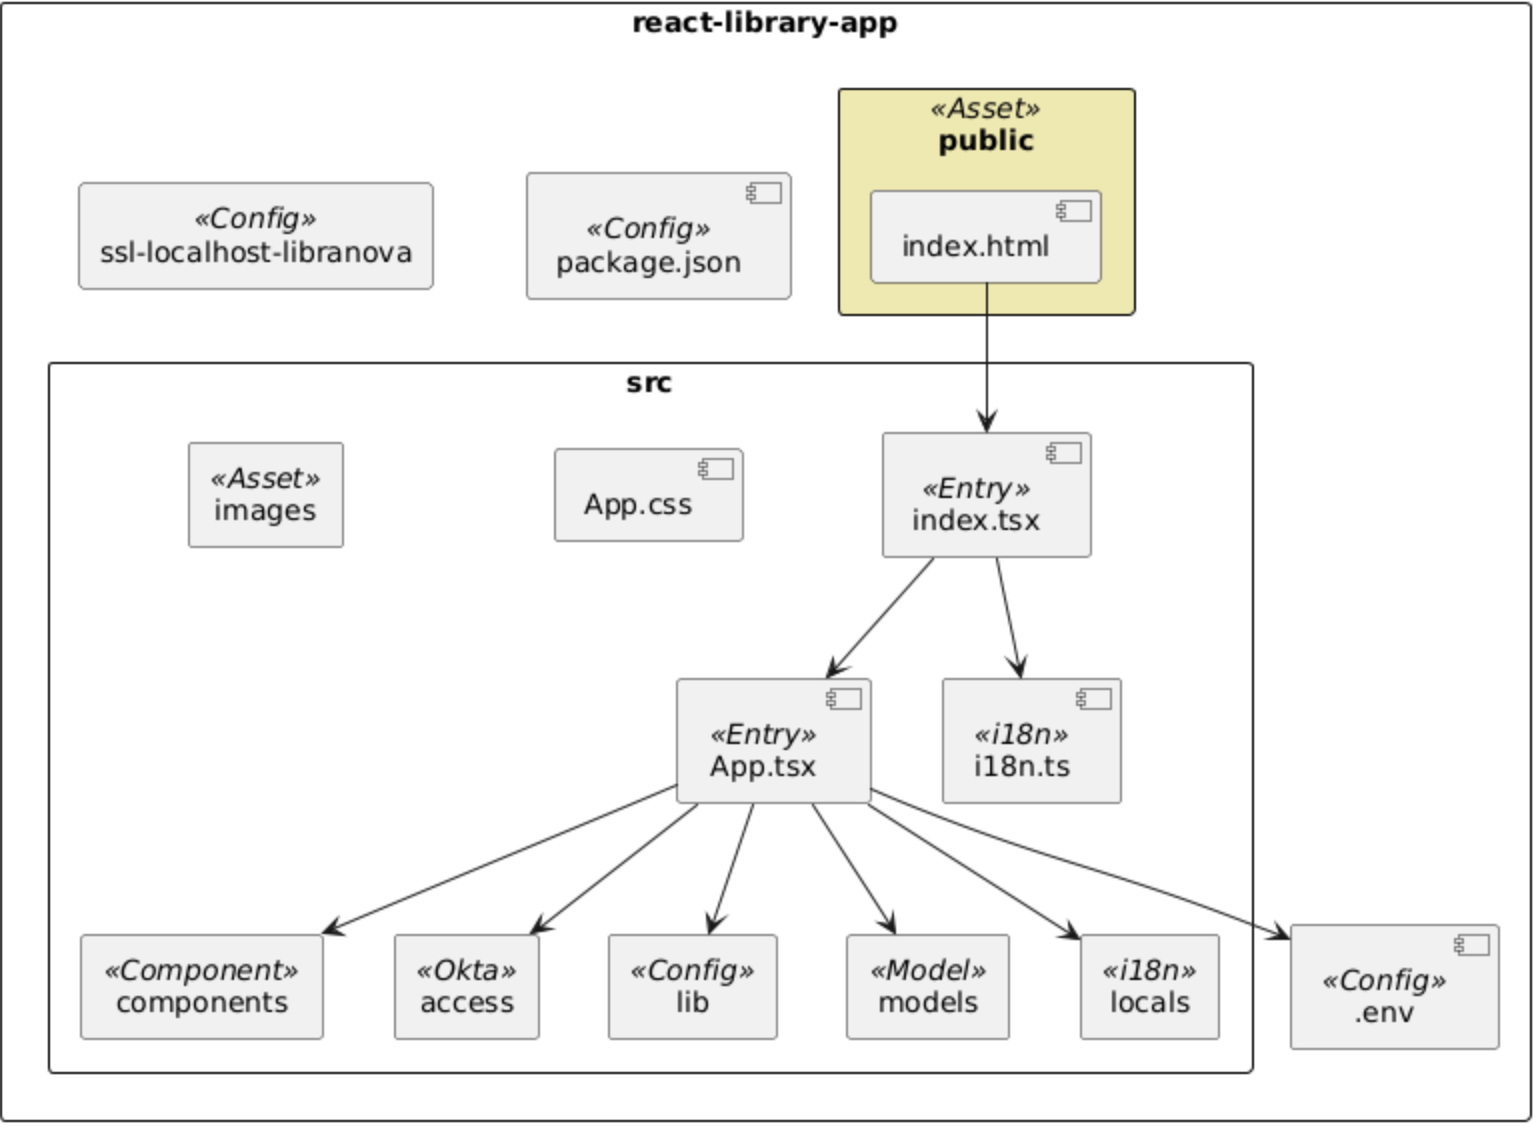
\includegraphics[width=1.00\textwidth]{images/frontend_structure.png}
	\caption{Modularer Aufbau des Frontends}
	\label{fig:folder-structure}
\end{figure} 
\noindent Anschließend werden die wichtigsten Ordner und Dateien sowie ihre jeweiligen Aufgabenbereiche beschrieben.
\begin{itemize}
	\item \textbf{index.html:} Statisches HTML-Grundgerüst der Anwendung. Enthält das \texttt{<div>} mit der ID \texttt{root}, in das React die App rendert. Zusätzlich werden hier externe Ressourcen wie Bootstrap und Stripe eingebunden.
	
	\item \textbf{package.json:} Zentrale Konfigurationsdatei für das React-Projekt. Definiert alle Projektabhängigkeiten, Skripte zur Ausführung (z.\,B.\ Starten, Bauen, Testen), sowie weitere Metadaten der Anwendung.
	
	\item \textbf{ssl-local-libranova:} Enthält SSL-Zertifikat (\texttt{localhost.crt}) und privaten Schlüssel (\texttt{localhost.key}) für die lokale HTTPS-Entwicklung.
	
	\item \textbf{index.tsx:} (siehe Listing~\ref{lst:react-index}) — bereits zuvor beschrieben im Abschnitt zur Einstiegspunktstruktur.
	
	\item \textbf{App.css:} Enthält benutzerdefinierte globale CSS-Regeln zur Gestaltung zentraler UI-Komponenten, darunter Header, Buttons, Bilder, Effekte sowie Media Queries zur responsiven Darstellung.
	
	\item \textbf{images:} Enthält statische Bilddateien, die in der Benutzeroberfläche verwendet werden.
	
	\item \textbf{i18n.ts:} Initialisiert die Mehrsprachigkeit mittels \texttt{i18next} mit englischen und deutschen Übersetzungen sowie automatischer Sprachenerkennung.
	
	\item \textbf{App.tsx:}  
	Zentrale Komponente der Anwendung, die das Routing und die Navigation steuert.  
	Sie bindet verschiedene Seiten und Komponenten ein und integriert die Authentifizierung mit Okta.  
	Header und Footer sorgen für das Layout, während geschützte Routen durch \texttt{Security} verwaltet werden.
	
	\item \textbf{components:}  
	Enthält die wiederverwendbaren UI-Komponenten der Anwendung, wie Header, Footer, Hauptseite, Suchseite und weitere funktionale Elemente.  
	Diese Komponenten bilden die Benutzeroberfläche und sind modular aufgebaut, um Wartbarkeit und Erweiterbarkeit zu gewährleisten.
	
	\item \textbf{access:}  
	Beinhaltet die Integration und Steuerung des Okta-Authentifizierungswidgets.  
	Die Komponenten \texttt{OktaLoginWidget} und \texttt{OktaSigninWidget} ermöglichen das Anmelden, Handhaben von Login-Events und Weiterleitung nach erfolgreicher Authentifizierung.  	
	
	\item \textbf{lib:}  
	Enthält die Datei \texttt{oktaConfig.ts}, die die Einstellungen für die Okta-Authentifizierung definiert, wie Client-ID, Autorisierungsserver (Issuer), Redirect-URI und Berechtigungen (Scopes).  
	Diese Konfiguration ist zentral für die Anbindung der Okta-Authentifizierung im Frontend.
	
	\item \textbf{models:}  
	Enthält Klassen, die zentrale Datenstrukturen der Anwendung modellieren, wie z.\,B. \texttt{Book}.  
	Sie dienen als Grundlage für den strukturierten Datenaustausch innerhalb des Frontends sowie zwischen Frontend und Backend.
	
	\item \textbf{locales:}  
	Beinhaltet sprachspezifische JSON-Dateien (\texttt{en}, \texttt{de}) für die Internationalisierung der UI mittels \texttt{react-i18next}.
	
	\item \textbf{.env:}  
	Diese Datei definiert Umgebungsvariablen für das Projekt.  
	Dazu gehören Pfade zu SSL-Zertifikat und -Schlüssel für die HTTPS-Kommunikation im lokalen Entwicklungsumfeld sowie die Backend-URL (\texttt{REACT\_APP\_API\_URL}) für die React-Anwendung.

\end{itemize}

\subsection{Internationalisierung mit i18next}\index{Internationalisierung mit i18next}

Zur Umsetzung der Mehrsprachigkeit im Frontend wurde das \texttt{i18next}-Framework in Kombination mit \texttt{react-i18next} und \texttt{i18next-browser-languagedetector} verwendet. Nach der Installation dieser Abhängigkeiten wird in der Datei \texttt{i18n.ts} (siehe Listing~\ref{lst:i18n.ts}) die Initialisierung des Übersetzungssystems vorgenommen.


\begin{lstlisting}[style=pseudocode, caption={Initialisierung von i18next in \texttt{i18n.ts}}, label={lst:i18n.ts}, breaklines=true]
import i18n from "i18next";
import { initReactI18next } from "react-i18next";
import LanguageDetector from "i18next-browser-languagedetector";

import translationEN from "./locales/en/translation.json";
import translationDE from "./locales/de/translation.json";

const resources = {
	en: { translation: translationEN },
	de: { translation: translationDE }
};

i18n
.use(LanguageDetector)  // Detektiert die Sprache des Benutzers
.use(initReactI18next) // Bindet i18next an React
.init({
	resources,
	fallbackLng: "en", // verwenden Sie Englisch als Fallback-Sprache
	interpolation: {
		escapeValue: false // React bereits vor XSS-Angriffen schützt
	}
});

export default i18n;
\end{lstlisting}

\noindent Hier ist eine Zeile-für-Zeile-Erklärung der Datei \texttt{i18n.ts}, die die Internationalisierung der React-Anwendung initialisiert:

\begin{itemize}
	\item \texttt{import i18n from "\texttt{i18next}";} \\
	Importiert die Hauptbibliothek \texttt{i18next}, die die Internationalisierung ermöglicht.
	
	\item \texttt{import \{ initReactI18next \} from "react-i18next";} \\
	Importiert die React-spezifische Integration, um \texttt{i18next} mit React zu verbinden.
	
	\item \texttt{import LanguageDetector from " \texttt{i18next}-browser-languagedetector";} \\
	Importiert ein Modul zur automatischen Erkennung der Sprache des Benutzers im Browser.
	
	\item \texttt{import translationEN from "./locales/en/translation.json";} \\
	Importiert die englischen Übersetzungen aus der JSON-Datei.
	
	\item \texttt{import translationDE from "./locales/de/translation.json";} \\
	Importiert die deutschen Übersetzungen aus der JSON-Datei.
	
	\item \texttt{const resources = \{} \\
	\hspace{1em} \texttt{en: \{ translation: translationEN \},} \\
	\hspace{1em} \texttt{de: \{ translation: translationDE \}} \\
	\texttt{\};} \\
	Definiert die verfügbaren Sprachressourcen mit den jeweiligen Übersetzungen.
	
	\item \texttt{i18n} \\
	\hspace{1em} \texttt{.use(LanguageDetector)} \\
	\hspace{1em} \texttt{.use(initReactI18next)} \\
	\hspace{1em} \texttt{.init(\{} \\
	\hspace{2em} \texttt{resources,} \\
	\hspace{2em} \texttt{fallbackLng: "en",} \\
	\hspace{2em} \texttt{interpolation: \{} \\
	\hspace{3em} \texttt{escapeValue: false} \\
	\hspace{2em} \texttt{\}} \\
	\hspace{1em} \texttt{\});} \\
	Initialisiert \texttt{i18next} mit: automatischer Spracherkennung, React-Integration, Sprachressourcen, Standard-Fallbacksprache Englisch, und deaktiviert Escape-Mechanismen, da React bereits sicher ist.
	
	\item \texttt{export default i18n;} \\
	Exportiert die konfigurierte Instanz, damit sie im Projekt verwendet werden kann.
\end{itemize}

\noindent Die sprachspezifischen Übersetzungen sind in den Ordnern \texttt{en} und \texttt{de} als strukturierte \texttt{.json}-Dateien organisiert.

\noindent Ein typisches Beispiel (siehe Listing~\ref{lst:use-translation}) für die Verwendung in einer React-Komponente ist:

\begin{lstlisting}[language=Java, caption={Beispielhafte Nutzung von \texttt{useTranslation}}, label={lst:use-translation}]
	import { useTranslation } from 'react-i18next';
	
	const { t } = useTranslation();
	
	<button>{t("checkout.thankYouReview")}</button>
\end{lstlisting}

\noindent In den entsprechenden JSON-Dateien sind die Übersetzungen wie folgt definiert:

\textbf{en.json:}
\begin{lstlisting}[style=pseudocode, caption={Englische Übersetzung in \texttt{en.json}}, label={lst:en-json-checkout}]
	"checkout": {
		"thankYouReview": "Thank you for your review"
	}
\end{lstlisting}

\textbf{de.json:}
\begin{lstlisting}[style=pseudocode, caption={Deutsche Übersetzung in \texttt{de.json}}, label={lst:de-json-checkout}]
	"checkout": {
		"thankYouReview": "Vielen Dank für deine Bewertung"
	}
\end{lstlisting}

\noindent Wie in Listing~\ref{lst:en-json-checkout} und Listing~\ref{lst:de-json-checkout} zu sehen, werden die Schlüssel \texttt{checkout.thankYouReview} mit den jeweiligen Texten in Englisch und Deutsch belegt.


\noindent Zur Laufzeit kann die Sprache über ein Dropdown-Menü gewechselt werden. Im Header.tsx  (siehe Listing~\ref{lst:language-switcher}) der Anwendung befindet sich ein Sprachumschalter, der die aktuelle Sprache visuell mit einem Icon anzeigt und dem Benutzer den Wechsel zwischen Deutsch und Englisch ermöglicht:

\begin{lstlisting}[style=pseudocode, caption={Sprachumschalter im Header}, label={lst:language-switcher}]
	<div className="dropdown">
	<button>
	{i18n.language === 'de' ? '[DE]' : '[EN]'}
	</button>
	<ul className="dropdown-menu">
	<li><button onClick={() => i18n.changeLanguage('en')}>[EN] English</button></li>
	<li><button onClick={() => i18n.changeLanguage('de')}>[DE] Deutsch</button></li>
	</ul>
	</div>
\end{lstlisting}

\noindent Hier ist die Zeilen-für-Zeilen-Erklärung des Sprachumschalters:
\begin{itemize}
	\item \texttt{\textless{}div className="dropdown"\textgreater{}}: Definiert einen Dropdown-Container für die Sprachwahl.
	\item \texttt{\textless{}button\textgreater{}}: Der Button zeigt die aktuell ausgewählte Sprache an.  
	Die Darstellung erfolgt dynamisch: Falls die Sprache Deutsch ist (\texttt{i18n.language === 'de'}), wird \texttt{[DE]} angezeigt, sonst \texttt{[EN]}.
	\item \texttt{\textless{}ul className="dropdown-menu"\textgreater{}}: Die Dropdown-Liste mit Sprachoptionen.
	\item \texttt{\textless{}li\textgreater{}\textless{}button onClick={() => i18n.changeLanguage('en')}\textgreater{}}: Ein Button zum Wechseln auf Englisch. Beim Klick wird die Sprache zu Englisch gewechselt.
	\item \texttt{\textless{}li\textgreater{}\textless{}button onClick={() => i18n.changeLanguage('de')}\textgreater{}}: Ein Button zum Wechseln auf Deutsch. Beim Klick wird die Sprache zu Deutsch gewechselt.
\end{itemize}

\noindent Damit wird gewährleistet, dass die Benutzeroberfläche abhängig von der gewählten Sprache dynamisch angepasst wird.


\section{Datenbankmodell und Persistenz}\index{Datenbankmodell und Persistenz}
In diesem Abschnitt werden das Datenbankschema sowie die Umsetzung der Datenpersistenz mit Spring Data und Hibernate erläutert.

\subsection{Datenbankschema}\index{Datenbankschema}

Die Anwendung verwendet ein relationales MySQL-Datenbanksystem zur Speicherung persistenter Informationen wie Bücher, Ausleihen, Zahlungen, Bewertungen und Nachrichten.

\noindent Die folgenden Tabellen wurden modelliert (siehe Abbildung~\ref{fig:er-model}):

\begin{itemize}
		\item \texttt{book}: Enthält Informationen zu Büchern, einschließlich Titel, Autor, Beschreibung, Kategorie, Bild sowie verfügbarer Exemplare.
	
	\item \texttt{checkout}: Repräsentiert aktive Ausleihen. Jede Ausleihe ist mit einem Benutzer (über die E-Mail-Adresse) und einem Buch (über \texttt{book\_id}) verknüpft. Enthält außerdem Ausleih- und Rückgabedatum.
	
	\item \texttt{review}: Enthält Nutzerbewertungen zu Büchern. Jede Bewertung ist einem Benutzer und einem Buch zugeordnet. Felder umfassen Bewertung (Zahl), Datum und Bewertungstext.
	
	\item \texttt{messages}: Dient der Kommunikation zwischen Benutzern und Administratoren. Enthält Fragen, Antworten sowie den Status (\texttt{closed}).
	
	\item \texttt{history}: Speichert vergangene Ausleihen. Hält Buchinformationen (z.\,B. Titel, Autor, Beschreibung, Bild) sowie Ausleih- und Rückgabedatum fest.
	
	\item \texttt{payment}: Speichert Zahlungsinformationen, einschließlich Betrag und E-Mail-Adresse des Benutzers.
\end{itemize}

\begin{figure}[H]
	\centering
	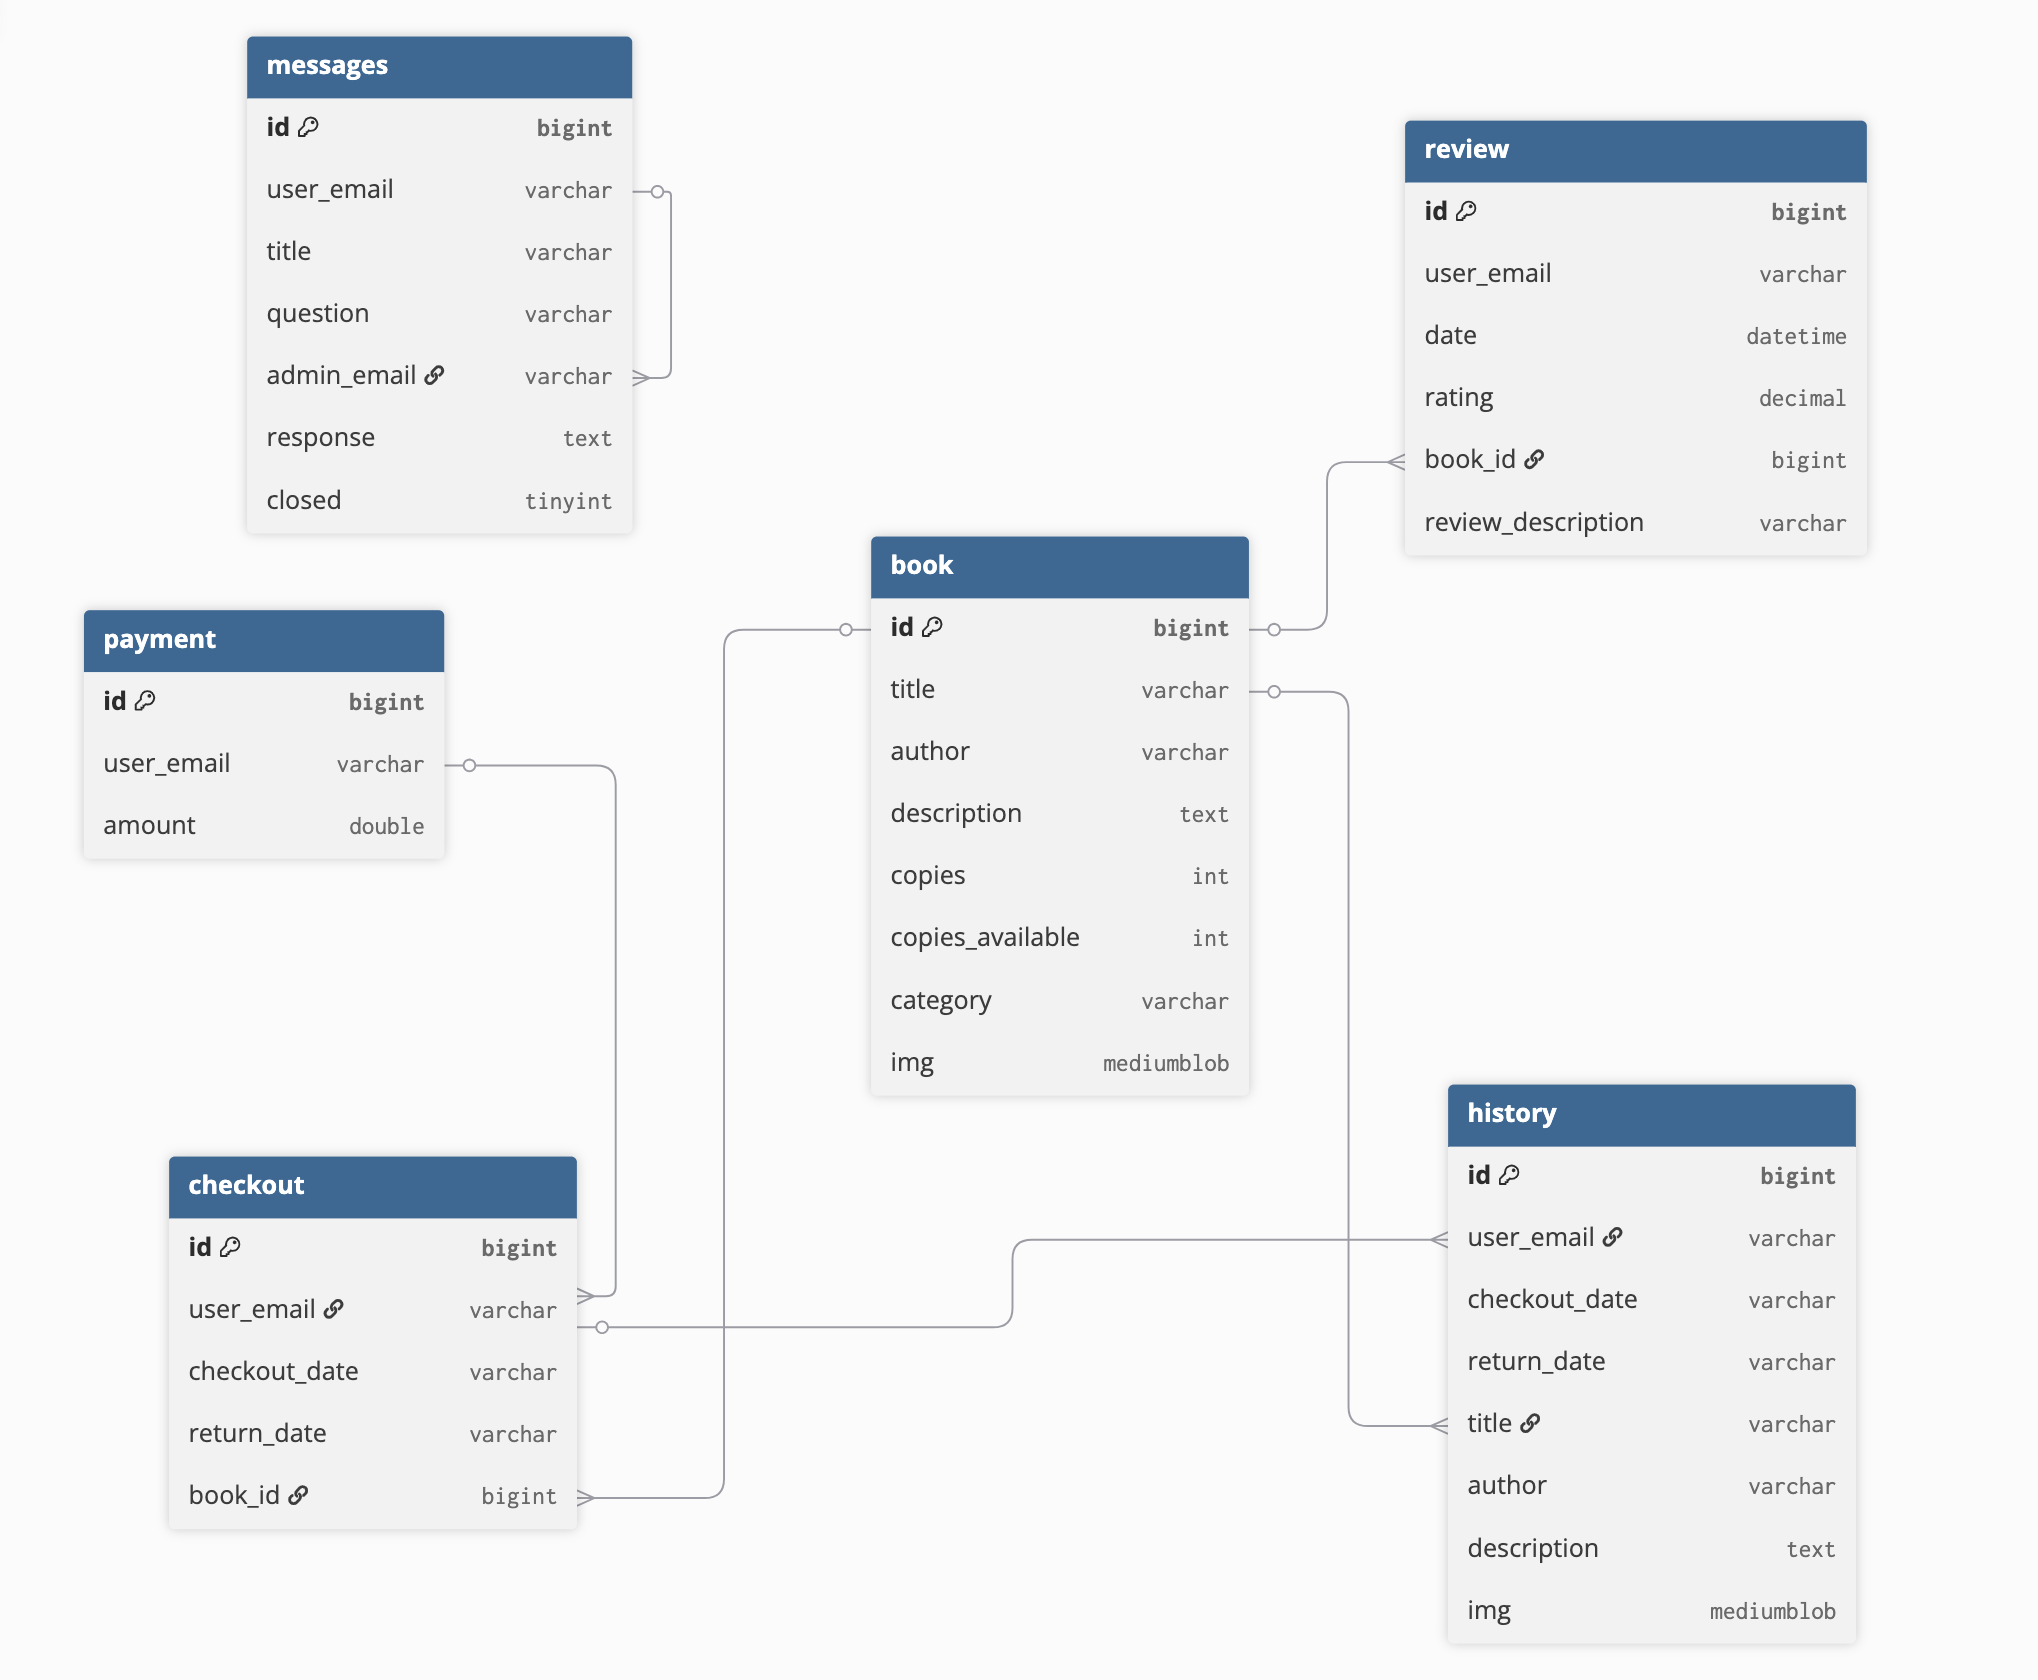
\includegraphics[width=0.99\textwidth]{images/DB-Schema.png}
	\caption{ER-Modell der Datenbank}
	\label{fig:er-model}
\end{figure}

\noindent Die logischen Beziehungen zwischen den Tabellen lassen sich wie folgt beschreiben:

\begin{itemize}
	\item Jede \texttt{checkout}-Instanz referenziert genau ein Buch über \texttt{book\_id}.
	\item Jede \texttt{review} ist einem Buch (book\_id) und einem Benutzer (user\_email) zugeordnet.
	\item Eine \texttt{message} verknüpft einen Benutzer mit einem Administrator über die jeweiligen E-Mail-Adressen.
	\item Ein \texttt{history}-Eintrag entspricht einer früheren Ausleihe eines Benutzers und speichert redundante Buchdaten.
	\item \texttt{payment}-Einträge entstehen nur bei verspäteter Rückgabe und sind über die Benutzer-E-Mail mit der Ausleihe verknüpft.
\end{itemize}


\subsection{Datenpersistenz mit Spring Data und Hibernate}\index{Datenpersistenz mit Spring Data und Hibernate}

Die Datenpersistenz wird mit Spring Boot in Verbindung mit Hibernate und Spring Data umgesetzt. Die Entitäten werden über Annotationen wie \texttt{@Entity}, \texttt{@Table}, \texttt{@Column}, \texttt{@Id}, und Beziehungen wie \texttt{@OneToMany} definiert.

\noindent Spring Data JPA und Spring Data REST übernehmen automatisch die Abbildung der Entitäten auf die Datenbanktabellen sowie die Bereitstellung von REST-APIs.

\noindent \textbf{Beispiel}: Entity-Klasse für Payments
\begin{lstlisting}[language=Java, caption={JPA-Entity \texttt{Payment}}, label={lst:Payment-entity}]
@Entity
@Table(name = "payment")
@Data
public class Payment {
	
	@Id
	@GeneratedValue(strategy = GenerationType.IDENTITY)
	private Long id;
	
	@Column(name = "user_email")
	private String userEmail;
	
	@Column(name = "amount")
	private double amount;
}
\end{lstlisting}

\noindent Diese Klasse stellt ein einfaches Beispiel für eine \texttt{Entity} dar, wie sie in Spring Data JPA und Hibernate verwendet wird. Die Annotationen übernehmen die automatische Zuordnung der Klasse zu einer Datenbanktabelle und ermöglichen eine saubere Trennung zwischen Domänenlogik und Datenpersistenz. Hier eine kurze Erklärung der wichtigsten Komponenten:

\begin{itemize}
	\item \texttt{@Entity}: Markiert die Klasse als JPA-Entity. Hibernate erkennt sie dadurch als persistente Klasse, die einer Tabelle in der Datenbank entspricht.
	
	\item \texttt{@Table(name = "payment")}: Gibt explizit an, dass die Klasse mit der Datenbanktabelle \texttt{payment} verknüpft ist. Falls die Annotation fehlt, würde standardmäßig der Klassenname als Tabellenname verwendet werden.
	
	\item \texttt{@Id}: Definiert das Feld \texttt{id} als Primärschlüssel der Tabelle.
	
	\item \texttt{@GeneratedValue(strategy = GenerationType.IDENTITY)}: Legt fest, dass der Primärschlüssel von der Datenbank automatisch (z.\,B.\ mittels AUTO\_INCREMENT) generiert wird. Dies ist typisch für MySQL.
	
	\item \texttt{@Column(name = "...")}: Weist jedes Attribut explizit einer Spalte in der Tabelle zu. Das ist besonders nützlich, wenn sich Feld- und Spaltennamen unterscheiden (z.\,B.\ \texttt{userEmail} $\rightarrow$ \texttt{user\_email}).
	
	\item \texttt{@Data} (aus Lombok): Generiert automatisch Getter, Setter, \texttt{equals()}, \texttt{hashCode()} und \texttt{toString()}-Methoden, um Boilerplate-Code zu vermeiden. Dies erhöht die Lesbarkeit und spart Entwicklungszeit.
\end{itemize}

\noindent \textbf{Beispiel}: Automatische Repository-Methoden mit Spring Data JPA and rest
\begin{lstlisting}[language=Java, caption={Payments-Repository-Schnittstelle}, label={lst:Payment-repo}]
public interface PaymentRepository extends JpaRepository<Payment, Long> {
	    Payment findByUserEmail(String userEmail);
}

\end{lstlisting}

\noindent Dieses Interface definiert die Datenzugriffsschicht für die \texttt{Payment}-Entität. Durch die Erweiterung von \texttt{JpaRepository<Payment, Long>} stellt Spring automatisch alle grundlegenden CRUD-Operationen bereit. \texttt{Payment} bezeichnet die Entitätsklasse, \texttt{Long} ist der Datentyp des Primärschlüssels.

\noindent Die Methode \texttt{findByUserEmail(String userEmail)} nutzt die Konventionen von Spring Data JPA: Anhand des Methodennamens erkennt Spring automatisch, dass nach dem Attribut \texttt{userEmail} gesucht werden soll, und generiert im Hintergrund die entsprechende SQL-Abfrage.

\noindent Da Spring Data REST als Abhängigkeit eingebunden ist, werden automatisch REST-Endpunkte für das Repository verfügbar gemacht – ohne dass man eigene Controller oder Services definieren muss. Die Endpunkte folgen dabei einer standardisierten Struktur:

\begin{itemize}
	\item \texttt{GET /payments} → Alle Zahlungen abrufen
	\item \texttt{POST /payments} → Neue Zahlung erstellen
	\item \texttt{GET /payments/1} → Zahlung mit ID 1 abrufen
	\item \texttt{DELETE /payments/1} → Zahlung mit ID 1 löschen
\end{itemize}

\noindent So ermöglichen Spring Data JPA und Spring Data REST gemeinsam eine saubere Trennung von Datenmodell und Zugriffsschicht – bei minimalem Implementierungsaufwand.


